\section{Ejercicio 1}
\subsection{El Problema}

Obtenemos un polígono simple de $N$ lados, descompuesto en $N - 2$ triángulos. Los vértices de los mismos son también vértices del polígono original, tal que dos triángulos cualesquiera no tienen un punto estrictamente interior en común, y de manera tal que la unión de todos los triángulos produce el polígono original.

Lo que debemos hacer es reconstruir el polígono original, devolviendo los $N$ vértices del mismo ordenados en sentido horario. Además debemos hacerlo en \O{N * log N}.

\subsection{Desarrollo}
\subsubsection{Inspiración divina}

Lo primero que hicimos fue darnos cuenta de lo siguiente:

\textit{Todo segmento entre par de vértices puede aparecer cero, una o dos veces como lado de un triángulo}. Veamos por qué esto es cierto.

Un par de vértices puede no aparecer como lado de un triángulo. Esto se debe a que la descomposición en triángulos no es única, por lo que en la descomposición provista un par de vértices puede no encontrarse unido.

\ig{Imagenes/ej1/Imagen_A.png}{Posibles inputs del problema}

En este imagen vemos claramente como en la izquierda AC no aparece como ningún lado del triángulo, pero si en la derecha.

Ahora, si el segmento cruza el polígono por dentro y aparece como un lado de un triángulo, entonces tiene un triángulo de cada lado.

\begin{figure}[H]\centering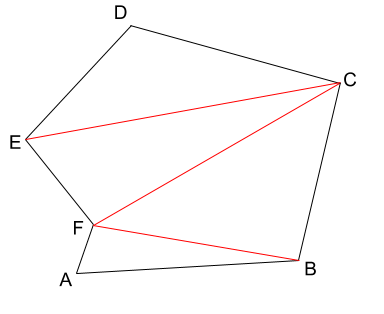
\includegraphics[scale=0.5]{Imagenes/ej1/Imagen_B.png}\caption{Segmentos internos}\end{figure}

Podemos ver como los segmentos BF, CF y CE tienen un triángulo a cada lado. Entonces dada la descomposición del polígono, cada segmento aparecerá 2 veces en distintos triángulos.

Finalmente, si el segmento es uno de los lados externos del polígono, solo tiene un triángulo del lado de adentro.

\begin{figure}[H]\centering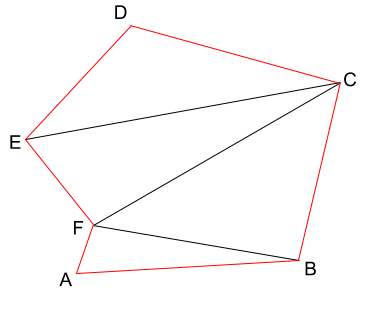
\includegraphics[scale=0.5]{Imagenes/ej1/Imagen_C.png}\caption{Lados externos del polígono}\end{figure}

Como vemos en la imagen, los lados externos del polígono solo pertenecen a un triángulo y por lo tanto aparecerán una vez en la descomposición.

\subsubsection{Solución}
Nuestra idea entonces es ir guardando los distintos lados de los triángulos que leemos. Pero, si encontramos uno ya guardado, lo borramos en vez de guardarlo. De esta forma, solo nos quedaríamos con los que aparecen una vez, es decir, los del polígono original.

\underline{\textbf{Implementación:}}

Dada la siguiente imagen, cuando leemos el triángulo ABF, para A guardamos B y F, para B, A y F, y para F, A y B

\begin{figure}[H]\centering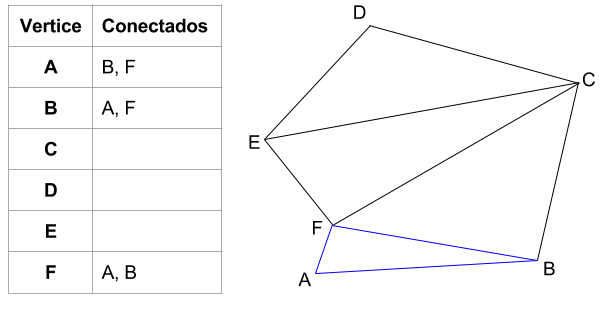
\includegraphics[scale=0.7]{Imagenes/ej1/Imagen_D.png}\caption{Lectura de ABF}\end{figure}

Cuando leamos el triángulo BCF, haremos lo mismo. Pero dado que B ya tenía guardado a F y viceversa, borraremos ambos vértices en vez de guardarlos.

\begin{figure}[H]\centering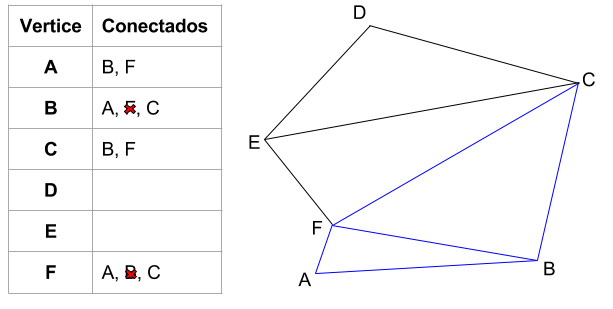
\includegraphics[scale=0.7]{Imagenes/ej1/Imagen_E.png}\caption{Lectura de BCF}\end{figure}

Una vez leídos todos los triángulos, nos quedaría lo siguiente:

\begin{figure}[H]\centering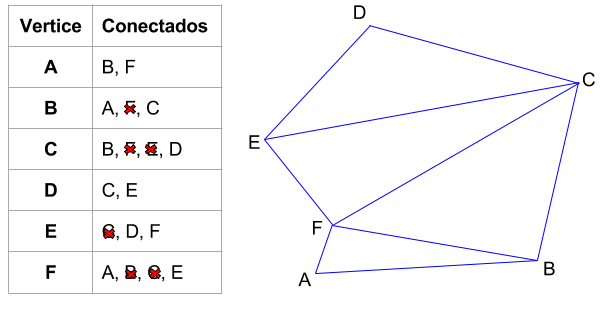
\includegraphics[scale=0.7]{Imagenes/ej1/Imagen_F.png}\caption{Todos los triángulos leídos}\end{figure}

Podemos ver que todos los vértices tienen solo a otros 2 conectados, y si prestamos atención nos damos cuenta que solo nos quedamos con los lados externos del polígono.

Después, tomamos el punto más a la izquierda y más abajo y elegimos el punto adyacente que respete el sentido horario. Dada nuestra última imagen, agarraríamos a \textit{E}, y tomaríamos como siguiente a \textit{D}. Desde ahí, es cuestión de ir recorriendo los puntos tomando desde cada punto aquél conectado que no fue el anterior. Una vez que volvimos a \textit{E}, terminamos.

\subsection{Complejidad}
El algoritmo en sí es bastante simple. La tabla vista en las imágenes es básicamente un vector con conjuntos adentro.

Cuando leemos los $N - 2$ triángulos, para cada vértice agregamos o quitamos los otros 2. Estas operaciones cuestan \O{log N} y las hacemos \O{N} veces. Por lo tanto la inicialización termina costando \O{N * log N}.

Luego, tenemos que ir recorriendo los vértices restantes e imprimirlos. Esto es solamente \O{N}, ya que cada vértice tiene solo otros 2 asociados. Cualquier decisión sobre elegir el siguiente vértice termina siendo \O{1}.

En conclusión, el algoritmo cuesta \O{N * log N} + \O{N} = \O{N * log N}.

\subsection{Puntaje}
El peso otorgado a este ejercicio es:
